\documentclass[11pt]{article}

% ── Packages ──────────────────────────────────────────────────────────────────
\usepackage[utf8]{inputenc}
\usepackage[T1]{fontenc}
\usepackage{amsmath,amssymb,amsthm}
\usepackage{graphicx}
\usepackage{booktabs}
\usepackage{multirow}
\usepackage{xcolor}
\usepackage{tikz}
\usetikzlibrary{arrows.meta, positioning, fit, backgrounds, matrix, shapes.geometric, decorations.pathreplacing}
\usepackage{colortbl}
\usepackage{pgfplots}
\pgfplotsset{compat=1.18}
\usepackage[a4paper, margin=1in]{geometry}
\usepackage[colorlinks=true, linkcolor=blue!60!black, citecolor=blue!60!black, urlcolor=blue!60!black]{hyperref}
\usepackage{microtype}
\usepackage{enumitem}

% ── Theorem environments ───────────────────────────────────────────────────────
\newtheorem{theorem}{Theorem}[section]
\newtheorem{definition}[theorem]{Definition}
\newtheorem{proposition}[theorem]{Proposition}

% ── Document ──────────────────────────────────────────────────────────────────
\title{%
  \textbf{Survey of Attention Mechanisms in\\
  Encoder-Only Language Models}
}
\author{
  Cristian Leo \\
  \textit{Independent} \\
  \texttt{cristianleo120@gmail.com}
  \and
  Daniel Begimher \\
  \textit{Independent} \\
  \texttt{bagaimher@gmail.com}
}
\date{March 2026}

\begin{document}
\maketitle

% ── Abstract ─────────────────────────────────────────────────────────────────
\begin{abstract}
The introduction of the Transformer architecture in 2017 catalyzed a fundamental paradigm shift in natural language processing~\cite{vaswani2017attention}. While decoder-only autoregressive models have come to dominate generative AI, encoder-only bidirectional models historically establish and maintain state-of-the-art results in natural language understanding, dense information retrieval, and sequence classification. This paper presents an exhaustive survey of the self-attention mechanism within encoder-only models. We analyze its mathematical foundations, trace its architectural evolution from the original BERT~\cite{devlin2018bert} through RoBERTa~\cite{liu2019roberta}, DeBERTa~\cite{he2020deberta}, and ModernBERT~\cite{warner2024smarter}, evaluate efficiency enhancements including sparse attention~\cite{zaheer2020big}, linear kernelized attention, and hardware-aware FlashAttention~\cite{dao2022flashattention}, and dissect the ongoing theoretical debates surrounding attention-based interpretability. We further survey hybrid architectures that interleave state-space models with self-attention, and discuss the practical limits and deployment considerations of encoder attention in long-context regimes.
\end{abstract}

\tableofcontents
\newpage

% ══════════════════════════════════════════════════════════════════════════════
\section{Introduction to the Encoder-Only Paradigm}
% ══════════════════════════════════════════════════════════════════════════════

The introduction of the Transformer by Vaswani et al.~\cite{vaswani2017attention} replaced the sequential processing bottlenecks of recurrent neural networks (RNNs) and long short-term memory (LSTM) networks with a highly parallelizable self-attention mechanism, enabling the direct modeling of long-range dependencies without vanishing gradients inherent in recurrence. The original dual encoder-decoder structure was designed specifically for sequence transduction such as machine translation; subsequent research bifurcated into two distinct lineages: decoder-only autoregressive models for generation, and encoder-only bidirectional models for understanding.

Encoder-only models—most prominently the Bidirectional Encoder Representations from Transformers (BERT)~\cite{devlin2018bert}—process the entire input sequence simultaneously without the causal masking required in autoregressive generation. Every token can attend to every other token in both directions, yielding deeply interconnected and semantically rich latent representations. These models are pre-trained via self-supervised objectives such as Masked Language Modeling (MLM)~\cite{devlin2018bert} that develop a profound understanding of syntax, semantics, and ontological relationships.

Despite the industry-wide pivot toward massive decoder-only LLMs, encoder-only architectures remain the most computationally efficient choice for discriminative tasks and embedding generation. However, the core bidirectional self-attention mechanism suffers from a quadratic computational complexity $\mathcal{O}(T^2)$ with respect to sequence length $T$, severely limiting applicability to long-context domains such as legal documents, medical records, or genomic sequences.

\subsection{Scope and Contributions}
This survey makes the following contributions:
\begin{enumerate}[label=(\roman*)]
  \item A rigorous mathematical treatment of bidirectional self-attention and its variants;
  \item A unified architectural taxonomy covering standard, disentangled, sparse, and linear attention paradigms;
  \item A critical review of hardware-aware optimizations (FlashAttention, FlexAttention);
  \item An analysis of hybrid SSM-Transformer encoder architectures;
  \item A synthesis of the interpretability debate and the attention-sink phenomenon; and
  \item Empirical benchmarks across GLUE, SuperGLUE, and dense retrieval with practical limits.
\end{enumerate}

% ══════════════════════════════════════════════════════════════════════════════
\section{Mathematical Foundations of Bidirectional Self-Attention}
% ══════════════════════════════════════════════════════════════════════════════

\subsection{Scaled Dot-Product Attention}

The core of the Transformer architecture is the attention mechanism, which allows for dynamic, content-based routing of information. In the context of bidirectional encoders, this mechanism is applied globally, enabling each token to integrate context from the entire sequence simultaneously. This operation fundamentally shifts the paradigm from recursive state updates (as in RNNs) to a direct, pairwise interaction model where path lengths between any two temporal positions are reduced to $\mathcal{O}(1)$.

\begin{definition}[Scaled Dot-Product Attention]
Given an input sequence $X \in \mathbb{R}^{T \times d_{\text{model}}}$, we first compute the linear projections:
\begin{equation}
  Q = XW_Q, \quad K = XW_K, \quad V = XW_V
\end{equation}
where $W_Q, W_K \in \mathbb{R}^{d_{\text{model}} \times d_k}$ and $W_V \in \mathbb{R}^{d_{\text{model}} \times d_v}$ are learnable weight matrices. The scaled dot-product attention is defined as:
\begin{equation}
  \text{Attention}(Q, K, V) = \text{softmax} \!\left( \frac{QK^\top}{\sqrt{d_k}} \right) V
  \label{eq:attention_formal}
\end{equation}
\end{definition}

\subsubsection{Intuition: Information Retrieval Analogy}
The mechanism can be conceptualized through the lens of information retrieval—a differentiable key-value store. A \textbf{query} $q_i$ (representing the $i$-th token's current state and searching intentions) is compared against a set of \textbf{keys} $\{k_1, \ldots, k_T\}$ (representing all tokens in the sequence and their available content) to determine their relevance. The dot product $q_i \cdot k_j$ serves as a similarity metric, measuring the alignment between the query's need and the key's offering. The resulting attention weights, normalized by the softmax function, determine how much of the information in the corresponding \textbf{values} $\{v_1, \ldots, v_T\}$ (the actual semantic payloads) is aggregated into the new representation of the $i$-th token. Consequently, each token transforms from a static embedding into a contextualized representation that encapsulates its role within the specific sequence.

The scaling factor $1/\sqrt{d_k}$ is critical for training stability. Without it, as the dimensionality $d_k$ increases, the magnitude of the dot products $QK^\top$ grows. Specifically, for independent random variables with zero mean and unit variance, their dot product has variance $d_k$. Large variances push the softmax function into regions where gradients approach zero, thus profoundly hindering backpropagation. The scaling restores the variance of the pre-softmax activations to $1$.

\subsubsection{Numerical Illustration}
To illustrate, consider a sequence of length $T=3$ with $d_k=4$. Let the query vector for the first token be $q_1 = [1, 0, 1, 0]$ and the key vectors for all tokens be:
\begin{equation*}
    K = \begin{bmatrix} 1 & 0 & 1 & 0 \\ 0 & 1 & 0 & 1 \\ 1 & 1 & 0 & 0 \end{bmatrix}
\end{equation*}
The raw dot products $q_1 K^\top$ would be $[2, 0, 1]$. Applying the scaling factor $\sqrt{d_k}=2$ yields $[1, 0, 0.5]$. After the softmax operation, we obtain weights $\approx [0.47, 0.17, 0.36]$. These weights dictate the linear combination of the value vectors $V$ that will form the output for the first token, showing how it ``attends'' primarily to itself and the third token. This explicit gating mechanism guarantees that extreme values are bounded and the output is a convex combination of the input values, maintaining the representation within a stable mathematical manifold.

\begin{figure}[ht]
\centering
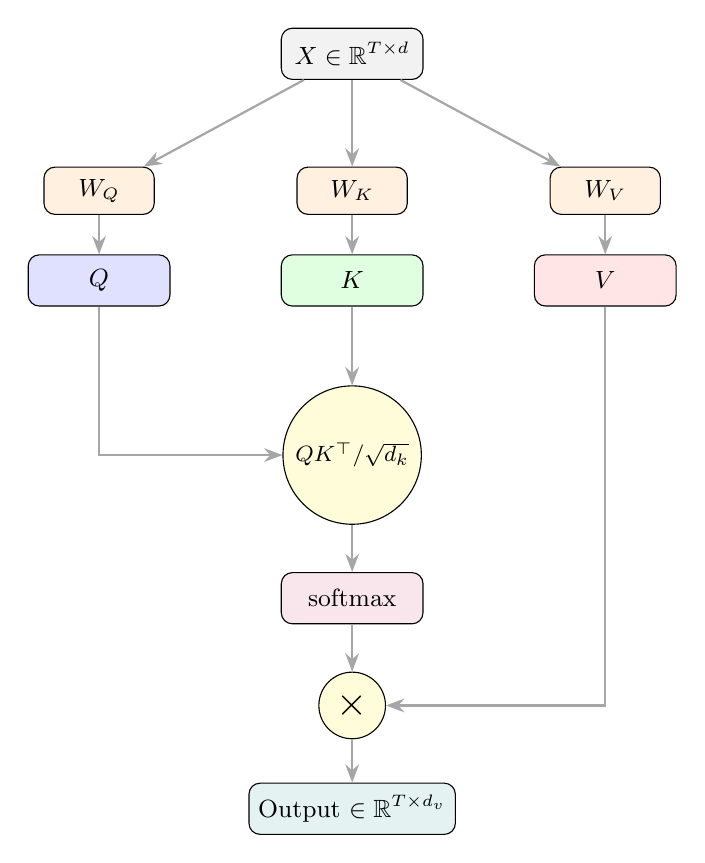
\begin{tikzpicture}[
  box/.style={draw, rounded corners=4pt, minimum width=1.8cm, minimum height=0.65cm,
               fill=blue!8, font=\small, align=center},
  matbox/.style={draw, rounded corners=4pt, minimum width=1.4cm, minimum height=0.6cm,
                 fill=orange!12, font=\small\itshape, align=center},
  arr/.style={-Stealth, thick, gray!70},
  every node/.style={font=\small}
]
  % Input X
  \node[box, fill=gray!10] (X) {$X \in \mathbb{R}^{T\times d}$};

  % Three projection branches
  \node[matbox, below left=1.1cm and 1.6cm of X]  (WQ) {$W_Q$};
  \node[matbox, below=1.1cm of X]                 (WK) {$W_K$};
  \node[matbox, below right=1.1cm and 1.6cm of X] (WV) {$W_V$};

  \node[box, fill=blue!12,  below=0.5cm of WQ] (Q) {$Q$};
  \node[box, fill=green!12, below=0.5cm of WK] (K) {$K$};
  \node[box, fill=red!10,   below=0.5cm of WV] (V) {$V$};

  % Dot-product node
  \node[draw, circle, fill=yellow!15, below=1.0cm of K,
        minimum size=0.9cm, font=\footnotesize, align=center] (dot) {$QK^\top / \sqrt{d_k}$};

  % Softmax
  \node[box, fill=purple!10, below=0.6cm of dot] (sm) {softmax};

  % Multiply by V
  \node[draw, circle, fill=yellow!15, below=0.6cm of sm,
        minimum size=0.7cm, font=\Large] (mul) {$\times$};

  % Output
  \node[box, fill=teal!10, below=0.55cm of mul] (out) {Output $\in\mathbb{R}^{T\times d_v}$};

  % Arrows from X to projections
  \draw[arr] (X) -- (WQ);
  \draw[arr] (X) -- (WK);
  \draw[arr] (X) -- (WV);

  % Projections to Q,K,V
  \draw[arr] (WQ) -- (Q);
  \draw[arr] (WK) -- (K);
  \draw[arr] (WV) -- (V);

  % Q,K into dot-product
  \draw[arr] (Q.south) |- (dot.west);
  \draw[arr] (K) -- (dot);

  % dot → softmax → multiply
  \draw[arr] (dot) -- (sm);
  \draw[arr] (sm) -- (mul);

  % V into multiply
  \draw[arr] (V.south) |- (mul.east);

  % multiply → output
  \draw[arr] (mul) -- (out);
\end{tikzpicture}
\caption{Scaled dot-product attention computation. The input sequence $X$ is linearly projected into query ($Q$), key ($K$), and value ($V$) spaces. Dot products between $Q$ and $K$ are scaled by $1/\sqrt{d_k}$ and normalized by softmax to produce attention weights, which then aggregate the values.}
\label{fig:attention_flow}
\end{figure}

\subsection{Multi-Head Attention}

The single-head attention mechanism is limited to a single mode of interaction, often causing a mixing of distinct semantic and syntactic signals. To capture diverse relationships concurrently, the mechanism is extended to multi-head attention (MHA). Instead of performing a single attention function in a $d_{\text{model}}$-dimensional space, the keys, values, and queries are linearly projected $h$ times with different, learned linear projections to $d_k$, $d_k$, and $d_v$ dimensions, respectively.

\begin{equation}
  \text{MultiHead}(Q, K, V) = \text{Concat}(\text{head}_1, \ldots, \text{head}_h) W^O
\end{equation}
where $\text{head}_i = \text{Attention}(Q W_i^Q, K W_i^K, V W_i^V)$ and $W^O \in \mathbb{R}^{h d_v \times d_{\text{model}}}$. By projecting $Q, K$, and $V$ into $h$ different subspaces, the model can simultaneously attend to different aspects of the input. For instance, one head might track subject-verb agreement while another resolves pronoun references, massively increasing the representational capacity without substantially expanding the parameter count.

\subsubsection{Functional Specialization of Heads}
Empirical studies of models like BERT have shown that different heads often specialize in distinct linguistic phenomena over the course of unsupervised pre-training. For example, some heads may focus on local syntactic structures (e.g., attending to the next token, the previous token, or the head of a dependency tree), while others capture global semantic relationships or act as ``attention sinks,'' attending primarily to separator tokens or punctuation. This redundancy and specialization are key to the robustness of Transformer representations. Pruning studies have even revealed that a large fraction of attention heads can be removed at inference time with minimal performance degradation, suggesting that while many heads are necessary for optimization, only a subset are critical for inference.

\subsection{Computational Complexity and Constraints}

\begin{proposition}[Quadratic Scaling]
Standard self-attention exhibits $\mathcal{O}(T^2 \cdot d)$ time complexity and $\mathcal{O}(T^2 \cdot h)$ space complexity.
\end{proposition}

The quadratic dependence on the sequence length $T$ arises from the materialization of the $T \times T$ attention matrix for each head. For a typical BERT model with $L=12$ layers and $h=12$ heads, the total number of attention entries for a sequence of length $T=512$ is $12 \times 12 \times 512^2 \approx 3.7 \times 10^7$ per forward pass. When processing longer sequences, the attention computation quickly dominates the feed-forward network (FFN) computation, transitioning the model from compute-bound to memory-bandwidth bound. Furthermore, during training, these matrices must be stored for backpropagation, making memory an even tighter bottleneck than compute.

% Fig 2 — Synthetic attention heatmap (explicit fills, no PGF array indexing)
\begin{figure}[ht]
\centering
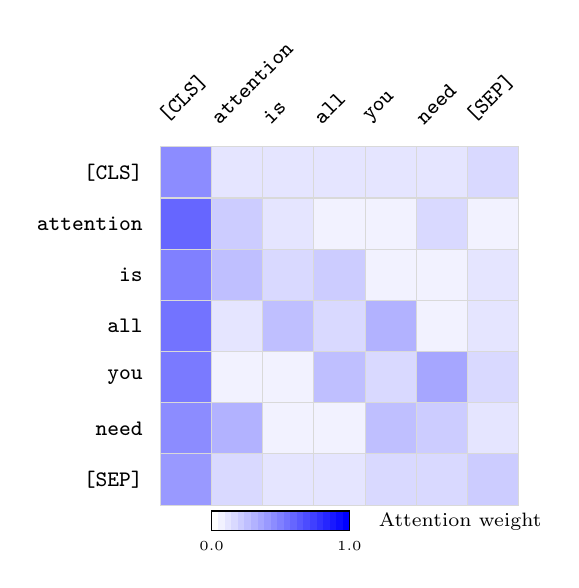
\begin{tikzpicture}
  \def\cs{0.65}
  
  % Row 0: [CLS]
  \fill[blue!45!white](0*\cs,-0*\cs)rectangle++(\cs,-\cs);\draw[gray!30,thin](0*\cs,-0*\cs)rectangle++(\cs,-\cs);
  \fill[blue!10!white](1*\cs,-0*\cs)rectangle++(\cs,-\cs);\draw[gray!30,thin](1*\cs,-0*\cs)rectangle++(\cs,-\cs);
  \fill[blue!10!white](2*\cs,-0*\cs)rectangle++(\cs,-\cs);\draw[gray!30,thin](2*\cs,-0*\cs)rectangle++(\cs,-\cs);
  \fill[blue!10!white](3*\cs,-0*\cs)rectangle++(\cs,-\cs);\draw[gray!30,thin](3*\cs,-0*\cs)rectangle++(\cs,-\cs);
  \fill[blue!10!white](4*\cs,-0*\cs)rectangle++(\cs,-\cs);\draw[gray!30,thin](4*\cs,-0*\cs)rectangle++(\cs,-\cs);
  \fill[blue!10!white](5*\cs,-0*\cs)rectangle++(\cs,-\cs);\draw[gray!30,thin](5*\cs,-0*\cs)rectangle++(\cs,-\cs);
  \fill[blue!15!white](6*\cs,-0*\cs)rectangle++(\cs,-\cs);\draw[gray!30,thin](6*\cs,-0*\cs)rectangle++(\cs,-\cs);
  
  % Row 1: attention
  \fill[blue!60!white](0*\cs,-1*\cs)rectangle++(\cs,-\cs);\draw[gray!30,thin](0*\cs,-1*\cs)rectangle++(\cs,-\cs);
  \fill[blue!20!white](1*\cs,-1*\cs)rectangle++(\cs,-\cs);\draw[gray!30,thin](1*\cs,-1*\cs)rectangle++(\cs,-\cs);
  \fill[blue!10!white](2*\cs,-1*\cs)rectangle++(\cs,-\cs);\draw[gray!30,thin](2*\cs,-1*\cs)rectangle++(\cs,-\cs);
  \fill[blue!5!white] (3*\cs,-1*\cs)rectangle++(\cs,-\cs);\draw[gray!30,thin](3*\cs,-1*\cs)rectangle++(\cs,-\cs);
  \fill[blue!5!white] (4*\cs,-1*\cs)rectangle++(\cs,-\cs);\draw[gray!30,thin](4*\cs,-1*\cs)rectangle++(\cs,-\cs);
  \fill[blue!15!white](5*\cs,-1*\cs)rectangle++(\cs,-\cs);\draw[gray!30,thin](5*\cs,-1*\cs)rectangle++(\cs,-\cs);
  \fill[blue!5!white] (6*\cs,-1*\cs)rectangle++(\cs,-\cs);\draw[gray!30,thin](6*\cs,-1*\cs)rectangle++(\cs,-\cs);
  
  % Row 2: is
  \fill[blue!50!white](0*\cs,-2*\cs)rectangle++(\cs,-\cs);\draw[gray!30,thin](0*\cs,-2*\cs)rectangle++(\cs,-\cs);
  \fill[blue!25!white](1*\cs,-2*\cs)rectangle++(\cs,-\cs);\draw[gray!30,thin](1*\cs,-2*\cs)rectangle++(\cs,-\cs);
  \fill[blue!15!white](2*\cs,-2*\cs)rectangle++(\cs,-\cs);\draw[gray!30,thin](2*\cs,-2*\cs)rectangle++(\cs,-\cs);
  \fill[blue!20!white](3*\cs,-2*\cs)rectangle++(\cs,-\cs);\draw[gray!30,thin](3*\cs,-2*\cs)rectangle++(\cs,-\cs);
  \fill[blue!5!white] (4*\cs,-2*\cs)rectangle++(\cs,-\cs);\draw[gray!30,thin](4*\cs,-2*\cs)rectangle++(\cs,-\cs);
  \fill[blue!5!white] (5*\cs,-2*\cs)rectangle++(\cs,-\cs);\draw[gray!30,thin](5*\cs,-2*\cs)rectangle++(\cs,-\cs);
  \fill[blue!10!white](6*\cs,-2*\cs)rectangle++(\cs,-\cs);\draw[gray!30,thin](6*\cs,-2*\cs)rectangle++(\cs,-\cs);
  
  % Row 3: all
  \fill[blue!55!white](0*\cs,-3*\cs)rectangle++(\cs,-\cs);\draw[gray!30,thin](0*\cs,-3*\cs)rectangle++(\cs,-\cs);
  \fill[blue!10!white](1*\cs,-3*\cs)rectangle++(\cs,-\cs);\draw[gray!30,thin](1*\cs,-3*\cs)rectangle++(\cs,-\cs);
  \fill[blue!25!white](2*\cs,-3*\cs)rectangle++(\cs,-\cs);\draw[gray!30,thin](2*\cs,-3*\cs)rectangle++(\cs,-\cs);
  \fill[blue!15!white](3*\cs,-3*\cs)rectangle++(\cs,-\cs);\draw[gray!30,thin](3*\cs,-3*\cs)rectangle++(\cs,-\cs);
  \fill[blue!30!white](4*\cs,-3*\cs)rectangle++(\cs,-\cs);\draw[gray!30,thin](4*\cs,-3*\cs)rectangle++(\cs,-\cs);
  \fill[blue!5!white] (5*\cs,-3*\cs)rectangle++(\cs,-\cs);\draw[gray!30,thin](5*\cs,-3*\cs)rectangle++(\cs,-\cs);
  \fill[blue!10!white](6*\cs,-3*\cs)rectangle++(\cs,-\cs);\draw[gray!30,thin](6*\cs,-3*\cs)rectangle++(\cs,-\cs);
  
  % Row 4: you
  \fill[blue!52!white](0*\cs,-4*\cs)rectangle++(\cs,-\cs);\draw[gray!30,thin](0*\cs,-4*\cs)rectangle++(\cs,-\cs);
  \fill[blue!5!white] (1*\cs,-4*\cs)rectangle++(\cs,-\cs);\draw[gray!30,thin](1*\cs,-4*\cs)rectangle++(\cs,-\cs);
  \fill[blue!5!white] (2*\cs,-4*\cs)rectangle++(\cs,-\cs);\draw[gray!30,thin](2*\cs,-4*\cs)rectangle++(\cs,-\cs);
  \fill[blue!25!white](3*\cs,-4*\cs)rectangle++(\cs,-\cs);\draw[gray!30,thin](3*\cs,-4*\cs)rectangle++(\cs,-\cs);
  \fill[blue!15!white](4*\cs,-4*\cs)rectangle++(\cs,-\cs);\draw[gray!30,thin](4*\cs,-4*\cs)rectangle++(\cs,-\cs);
  \fill[blue!35!white](5*\cs,-4*\cs)rectangle++(\cs,-\cs);\draw[gray!30,thin](5*\cs,-4*\cs)rectangle++(\cs,-\cs);
  \fill[blue!15!white](6*\cs,-4*\cs)rectangle++(\cs,-\cs);\draw[gray!30,thin](6*\cs,-4*\cs)rectangle++(\cs,-\cs);

  % Row 5: need
  \fill[blue!45!white](0*\cs,-5*\cs)rectangle++(\cs,-\cs);\draw[gray!30,thin](0*\cs,-5*\cs)rectangle++(\cs,-\cs);
  \fill[blue!30!white](1*\cs,-5*\cs)rectangle++(\cs,-\cs);\draw[gray!30,thin](1*\cs,-5*\cs)rectangle++(\cs,-\cs);
  \fill[blue!5!white] (2*\cs,-5*\cs)rectangle++(\cs,-\cs);\draw[gray!30,thin](2*\cs,-5*\cs)rectangle++(\cs,-\cs);
  \fill[blue!5!white] (3*\cs,-5*\cs)rectangle++(\cs,-\cs);\draw[gray!30,thin](3*\cs,-5*\cs)rectangle++(\cs,-\cs);
  \fill[blue!25!white](4*\cs,-5*\cs)rectangle++(\cs,-\cs);\draw[gray!30,thin](4*\cs,-5*\cs)rectangle++(\cs,-\cs);
  \fill[blue!20!white](5*\cs,-5*\cs)rectangle++(\cs,-\cs);\draw[gray!30,thin](5*\cs,-5*\cs)rectangle++(\cs,-\cs);
  \fill[blue!10!white](6*\cs,-5*\cs)rectangle++(\cs,-\cs);\draw[gray!30,thin](6*\cs,-5*\cs)rectangle++(\cs,-\cs);

  % Row 6: [SEP]
  \fill[blue!40!white](0*\cs,-6*\cs)rectangle++(\cs,-\cs);\draw[gray!30,thin](0*\cs,-6*\cs)rectangle++(\cs,-\cs);
  \fill[blue!15!white](1*\cs,-6*\cs)rectangle++(\cs,-\cs);\draw[gray!30,thin](1*\cs,-6*\cs)rectangle++(\cs,-\cs);
  \fill[blue!10!white](2*\cs,-6*\cs)rectangle++(\cs,-\cs);\draw[gray!30,thin](2*\cs,-6*\cs)rectangle++(\cs,-\cs);
  \fill[blue!10!white](3*\cs,-6*\cs)rectangle++(\cs,-\cs);\draw[gray!30,thin](3*\cs,-6*\cs)rectangle++(\cs,-\cs);
  \fill[blue!15!white](4*\cs,-6*\cs)rectangle++(\cs,-\cs);\draw[gray!30,thin](4*\cs,-6*\cs)rectangle++(\cs,-\cs);
  \fill[blue!15!white](5*\cs,-6*\cs)rectangle++(\cs,-\cs);\draw[gray!30,thin](5*\cs,-6*\cs)rectangle++(\cs,-\cs);
  \fill[blue!20!white](6*\cs,-6*\cs)rectangle++(\cs,-\cs);\draw[gray!30,thin](6*\cs,-6*\cs)rectangle++(\cs,-\cs);

  % Column labels (Keys)
  \node[font=\footnotesize\ttfamily,rotate=45,anchor=south west]at(0*\cs+0.1,0.1){[CLS]};
  \node[font=\footnotesize\ttfamily,rotate=45,anchor=south west]at(1*\cs+0.1,0.1){attention};
  \node[font=\footnotesize\ttfamily,rotate=45,anchor=south west]at(2*\cs+0.1,0.1){is};
  \node[font=\footnotesize\ttfamily,rotate=45,anchor=south west]at(3*\cs+0.1,0.1){all};
  \node[font=\footnotesize\ttfamily,rotate=45,anchor=south west]at(4*\cs+0.1,0.1){you};
  \node[font=\footnotesize\ttfamily,rotate=45,anchor=south west]at(5*\cs+0.1,0.1){need};
  \node[font=\footnotesize\ttfamily,rotate=45,anchor=south west]at(6*\cs+0.1,0.1){[SEP]};
  % Row labels (Queries)
  \node[font=\footnotesize\ttfamily,anchor=east]at(-0.1,-0*\cs-0.5*\cs){[CLS]};
  \node[font=\footnotesize\ttfamily,anchor=east]at(-0.1,-1*\cs-0.5*\cs){attention};
  \node[font=\footnotesize\ttfamily,anchor=east]at(-0.1,-2*\cs-0.5*\cs){is};
  \node[font=\footnotesize\ttfamily,anchor=east]at(-0.1,-3*\cs-0.5*\cs){all};
  \node[font=\footnotesize\ttfamily,anchor=east]at(-0.1,-4*\cs-0.5*\cs){you};
  \node[font=\footnotesize\ttfamily,anchor=east]at(-0.1,-5*\cs-0.5*\cs){need};
  \node[font=\footnotesize\ttfamily,anchor=east]at(-0.1,-6*\cs-0.5*\cs){[SEP]};
  % Colour bar (positioned below)
  \begin{scope}[shift={(1.0*\cs, -7.5*\cs)}]
    \foreach \x in {0,5,...,100} {
      \fill[blue!\x!white] (\x/60, 0) rectangle ++(5/60, 0.25);
    }
    \draw (0,0) rectangle (105/60, 0.25);
    \node[font=\tiny] at (0, -0.2) {0.0};
    \node[font=\tiny] at (105/60, -0.2) {1.0};
    \node[font=\scriptsize, anchor=west] at (2.0, 0.12) {Attention weight};
  \end{scope}
\end{tikzpicture}
\caption{Illustrative bidirectional self-attention heatmap (Layer~1, Head~1) for the sentence ``attention is all you need''. Colour intensity encodes the softmax attention weight from each row token (query) to each column token (key). The \texttt{[CLS]} token absorbs disproportionate probability mass, illustrating the attention sink effect.}
\label{fig:heatmap}
\end{figure}

This quadratic bottleneck is particularly acute in memory consumption. During training, the attention matrices must be stored for the backward pass, leading to $\mathcal{O}(L \cdot h \cdot T^2)$ memory requirements. This limitation motivates the architectural innovations discussed in Section~\ref{sec:taming}, which aim to sparsify or linearize the attention mechanism.

% ══════════════════════════════════════════════════════════════════════════════
\section{Architectural Evolution of Foundational Encoders}
% ══════════════════════════════════════════════════════════════════════════════

\subsection{BERT: Bidirectional Pre-Training at Scale}

Devlin et al.\ introduced BERT~\cite{devlin2018bert} as the first large-scale empirical validation of bidirectional attention for language understanding. BERT-Base employs 12 Transformer encoder blocks with 12 attention heads and a hidden dimension $d = 768$ (110M parameters); BERT-Large uses 24 blocks, 16 heads, and $d = 1024$ (340M parameters). Pre-training proceeds on 16 GB of raw text via two objectives that rely heavily on specialized functional tokens (\texttt{[CLS]}, \texttt{[SEP]}, and \texttt{[MASK]}):
\begin{itemize}
  \item \textbf{Masked Language Modeling (MLM):} BERT addresses the ``leakage'' problem in bidirectional training by masking 15\% of input tokens using the \texttt{[MASK]} token. The attention mechanism is forced to reconstruct these masked tokens by aggregating information from both leftward and rightward contexts simultaneously. Unlike causal models where attention is restricted to preceding tokens, MLM leverages the full $T \times T$ attention matrix to build a holistic representation of each token based on its entire surroundings. 
  
  \textit{Example MLM operation:} Given the original text \textit{``the dog barks loudly''}, the model might receive the input sequence \texttt{the dog [MASK] loudly}. The model is tasked with outputting the target word \textit{``barks''} at the position of the \texttt{[MASK]} token. To mitigate the discrepancy between pre-training and fine-tuning (where \texttt{[MASK]} does not appear), the model follows an 80-10-10 strategy: 80\% are replaced with \texttt{[MASK]}, 10\% with a random token, and 10\% remain unchanged. This forces attention heads to maintain accurate representations of all tokens, not just those explicitly marked as masked.
  
  \item \textbf{Next Sentence Prediction (NSP):} This objective is designed to teach the model cross-sentence relationships. Two sentences, $S_A$ and $S_B$, are concatenated with a \texttt{[SEP]} token as a structural boundary. The \texttt{[CLS]} token, prepended to the sequence, acts as a global attention sink that attends to every token in both $S_A$ and $S_B$. By aggregating this document-level context through all $L$ layers, the final hidden state of \texttt{[CLS]} captures the semantic coherence between the two segments, allowing the model to predict whether $S_B$ logically follows $S_A$.
  
  \textit{Example NSP operations:}
  \begin{itemize}
      \item \textbf{IsNext}: \texttt{[CLS] the man went to the store. [SEP] he bought a gallon of milk. [SEP]} $\rightarrow$ \texttt{True}
      \item \textbf{NotNext}: \texttt{[CLS] the man went to the store. [SEP] penguins are flightless birds. [SEP]} $\rightarrow$ \texttt{False}
  \end{itemize}
\end{itemize}

\begin{figure}[ht]
\centering
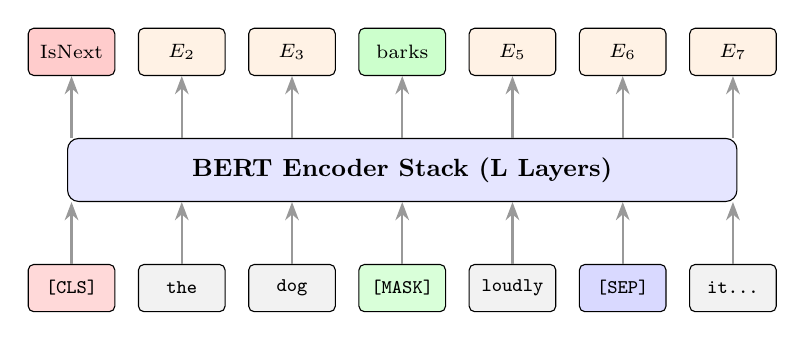
\begin{tikzpicture}[
  token/.style={draw, rounded corners=2pt, minimum width=1.1cm, minimum height=0.6cm, fill=gray!10, font=\scriptsize\ttfamily, align=center},
  enc/.style={draw, rounded corners=4pt, minimum width=8.5cm, minimum height=0.8cm, fill=blue!10, font=\small\bfseries, align=center},
  outblock/.style={draw, rounded corners=2pt, minimum width=1.1cm, minimum height=0.6cm, fill=orange!10, font=\scriptsize, align=center},
  arr/.style={-Stealth, thick, gray!80}
]
  % Input tokens
  \node[token, fill=red!15] (t1) at (0,0) {[CLS]};
  \node[token] (t2) at (1.4,0) {the};
  \node[token] (t3) at (2.8,0) {dog};
  \node[token, fill=green!15] (t4) at (4.2,0) {[MASK]};
  \node[token] (t5) at (5.6,0) {loudly};
  \node[token, fill=blue!15] (t6) at (7.0,0) {[SEP]};
  \node[token] (t7) at (8.4,0) {it...};

  % Encoder Stack
  \node[enc] (bert) at (4.2, 1.5) {BERT Encoder Stack (L Layers)};
  
  % Outputs
  \node[outblock, fill=red!20] (o1) at (0,3.0) {IsNext};
  \node[outblock] (o2) at (1.4,3.0) {$E_2$};
  \node[outblock] (o3) at (2.8,3.0) {$E_3$};
  \node[outblock, fill=green!20] (o4) at (4.2,3.0) {barks};
  \node[outblock] (o5) at (5.6,3.0) {$E_5$};
  \node[outblock] (o6) at (7.0,3.0) {$E_6$};
  \node[outblock] (o7) at (8.4,3.0) {$E_7$};

  % Connections
  \foreach \i in {1,...,7} {
    \draw[arr] (t\i) -- (t\i |- bert.south);
    \draw[arr] (t\i |- bert.north) -- (o\i);
  }
\end{tikzpicture}
\caption{BERT pre-training architecture. The \texttt{[CLS]} token produces the NSP classification, while the \texttt{[MASK]} token is used to predict the missing vocabulary word. The \texttt{[SEP]} token delimits the two sequence segments and marks the end of the input.}
\label{fig:bert_arch}
\end{figure}

BERT established state-of-the-art across 11 NLP tasks upon publication, cementing the validity of the bidirectional pre-training paradigm.

\subsection{RoBERTa: Optimizing the Training Recipe}

Liu et al.~\cite{liu2019roberta} demonstrated that BERT was significantly undertrained. RoBERTa matches the original BERT architecture but introduces: (i) a ten-fold increase in training data (160 GB), (ii) dynamic masking that generates novel mask patterns each epoch rather than using static masks, (iii) removal of the NSP objective (shown to degrade performance on downstream tasks), and (iv) larger batch sizes (up to 8,000 sequences).

\subsubsection{Scientific Impact of Scale on Attention Training}
The massive influx of training data (160 GB vs. BERT's 16 GB), coupled with dynamic masking, fundamentally altered the convergence trajectory of the attention heads. In standard BERT, the use of static masks across epochs allowed certain attention heads to collapse into trivial memorization patterns—essentially learning static positional offsets to reconstruct the fixed, repeatedly seen masked sequences. By dynamically regenerating masks at each epoch and exposing the model to an order of magnitude more syntactic variance, RoBERTa forcefully prevented this positional overfitting. Scientifically, this increased data variance acted as a potent regularizer on the attention landscape. The heads were forced to learn robust, generalized semantic routing strategies capable of handling unprecedented contexts, rather than relying on brittle, localized dependencies. Consequently, without modifying the core attention equations, RoBERTa's attention distributions became measurably sharper and more syntactically accurate, substantially improving performance on all benchmarks.

\begin{figure}[ht]
\centering
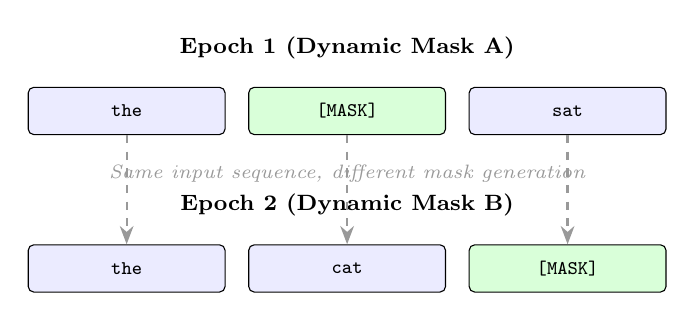
\begin{tikzpicture}[
  box/.style={draw, rounded corners=2pt, minimum width=2.5cm, minimum height=0.6cm, fill=blue!8, font=\scriptsize\ttfamily, align=center},
  mask/.style={draw, rounded corners=2pt, minimum width=2.5cm, minimum height=0.6cm, fill=green!15, font=\scriptsize\ttfamily\bfseries, align=center},
  arr/.style={-Stealth, thick, gray!80}
]
  \node[font=\footnotesize\bfseries] (e1) at (0, 2) {Epoch 1 (Dynamic Mask A)};
  \node[box] (t11) at (-2.8, 1.2) {the};
  \node[mask] (t12) at (0, 1.2) {[MASK]};
  \node[box] (t13) at (2.8, 1.2) {sat};

  \node[font=\footnotesize\bfseries] (e2) at (0, 0) {Epoch 2 (Dynamic Mask B)};
  \node[box] (t21) at (-2.8, -0.8) {the};
  \node[box] (t22) at (0, -0.8) {cat};
  \node[mask] (t23) at (2.8, -0.8) {[MASK]};
  
  \node[font=\scriptsize\itshape, text=gray!80] at (0, 0.4) {Same input sequence, different mask generation};

  \draw[arr, dashed] (t11.south) -- (t21.north);
  \draw[arr, dashed] (t12.south) -- (t22.north);
  \draw[arr, dashed] (t13.south) -- (t23.north);
\end{tikzpicture}
\caption{RoBERTa's Dynamic Masking. Instead of using a static mask for every epoch (as in BERT), the mask is generated dynamically. This forces attention heads to constantly adapt to new, unseen contextual contexts, significantly improving the robustness of the learned representations.}
\label{fig:roberta_dynamic}
\end{figure}

\subsection{ALBERT: Parameter-Efficient Factorization}

ALBERT~\cite{lan2019albert} addresses BERT's memory footprint via structural changes that radically alter the model's parameterization, even as it preserves the $\mathcal{O}(T^2)$ dense attention computation. Two primary mechanisms are employed:

\textbf{Cross-Layer Parameter Sharing:} In a standard BERT model, each layer $l \in [1, L]$ possesses its own independent attention weight matrices $\{W_Q^l, W_K^l, W_V^l, W_O^l\}$. ALBERT enforces weight sharing across all layers:
\begin{equation}
  W_Q^1 = W_Q^2 = \dots = W_Q^L
\end{equation}
This recursive application of the same attention parameters effectively transforms the deep stack of encoder layers into a single, iteratively refined transformation. While this drastically reduces the parameter count (achieving an 89\% reduction when comparing ALBERT-base to the equivalent BERT-base configuration), it increases the computational difficulty, as the same weights must generalize across the entire depth of the network.

\textbf{Factorized Embedding Parameterization:} ALBERT decomposes the large token embedding matrix into two smaller matrices. Rather than projecting directly from the vocabulary $V$ to the model dimension $d$, it first projects to a lower-dimensional space $E$, such that the total parameters are reduced from $\mathcal{O}(V \times d)$ to $\mathcal{O}(V \times E + E \times d)$. This allows the model dimension $d$ to grow significantly without a corresponding explosion in vocabulary-related parameters.

These architectural optimizations, combined with a Sentence-Order Prediction (SOP) loss to replace BERT's NSP, allow ALBERT to scale to much larger model dimensions while maintaining a lightweight footprint, albeit with a higher training time per parameter.

\begin{figure}[ht]
\centering
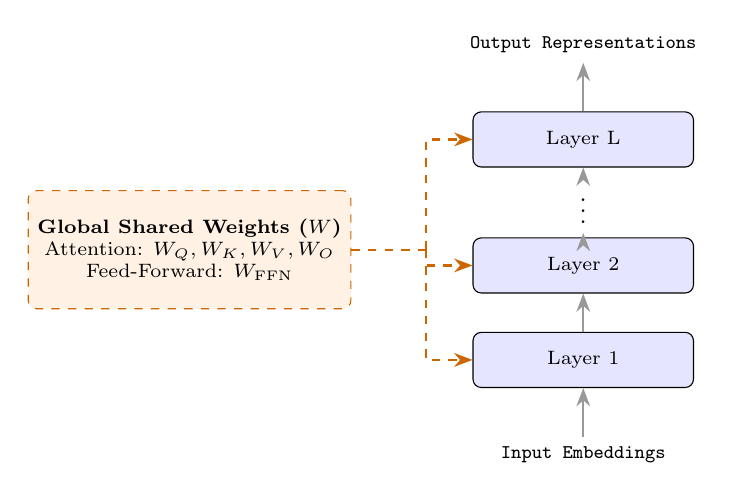
\begin{tikzpicture}[
  enc/.style={draw, rounded corners=3pt, minimum width=2.8cm, minimum height=0.7cm, font=\scriptsize, align=center},
  param/.style={draw=orange!80!black, dashed, rounded corners=3pt, minimum width=3.2cm, minimum height=1.5cm, fill=orange!10, font=\scriptsize, align=center},
  tok/.style={font=\scriptsize\ttfamily},
  arr/.style={-Stealth, thick, gray!80},
  paramarr/.style={-Stealth, thick, orange!80!black, dashed}
]

  % Global Parameters Block
  \node[param] (w) at (-3, 2.6) {\textbf{Global Shared Weights ($W$)}\\Attention: $W_Q, W_K, W_V, W_O$\\Feed-Forward: $W_{\text{FFN}}$};

  % Unrolled Layers
  \node[tok] (a_in)  at (2, 0) {Input Embeddings};
  \node[enc, fill=blue!10] (a1) at (2, 1.2) {Layer 1};
  \node[enc, fill=blue!10] (a2) at (2, 2.4) {Layer 2};
  \node[font=\small] (adots)  at (2, 3.2) {$\vdots$};
  \node[enc, fill=blue!10]   (aL) at (2, 4.0) {Layer L};
  
  \node[tok] (a_out) at (2, 5.2) {Output Representations};

  % Data flow
  \draw[arr] (a_in) -- (a1);
  \draw[arr] (a1) -- (a2);
  \draw[arr] (a2) -- (adots);
  \draw[arr] (adots) -- (aL);
  \draw[arr] (aL) -- (a_out);

  % Weight sharing arrows via orthogonal bus to prevent overlapping
  \coordinate (w_bus) at (0, 2.6);
  \draw[thick, orange!80!black, dashed] (w.east) -- (w_bus);
  \draw[paramarr] (w_bus) |- (a1.west);
  \draw[paramarr] (w_bus) |- (a2.west);
  \draw[paramarr] (w_bus) |- (aL.west);

\end{tikzpicture}
\caption{Cross-layer parameter sharing in ALBERT. Unlike standard architectures that instantiate independent weights for each layer, ALBERT maintains a single globally shared set of parameters ($W$) that is recurrently injected into every Transformer layer during the forward and backward passes.}
\label{fig:albert_sharing}
\end{figure}

\subsection{ELECTRA: Sampling-Efficient Discriminative Pre-Training}

Clark et al.~\cite{clark2020electra} proposed Replaced Token Detection (RTD) as a more sample-efficient alternative to the standard MLM objective. While the internal attention mechanism remains standard dot-product MHA, the training paradigm is radically altered to improve learning efficiency.

\textbf{Generator-Discriminator Architecture:} ELECTRA utilizes a two-network setup consisting of a small \emph{generator} ($G$) and a large \emph{discriminator} ($D$). The generator is typically a smaller BERT-style encoder (e.g., 1/4 the size of the discriminator) trained via standard MLM. It proposes plausible replacements for masked tokens based on its bidirectional context. The discriminator then attempts to predict, for \emph{every} token in the sequence, whether it is an ``original'' token or a ``replaced'' token generated by $G$.

\textbf{Sample Efficiency through Global Loss:} In standard BERT, the model only receives a training signal from the 15\% of tokens that are masked. In ELECTRA, the discriminator produces a binary classification for \emph{all} $T$ tokens. This means that every single token in every sequence participates in the final loss calculation, regardless of whether it was actually replaced. This dense training signal allows ELECTRA to reach the same level of performance as RoBERTa with significantly fewer FLOPs (approximately 1/4 of the compute).

While the generator is discarded after pre-training, the discriminator becomes the final encoder used for downstream tasks. Its attention heads, having been forced to detect extremely subtle semantic and syntactic anomalies produced by the generator, often exhibit higher sensitivity to nuanced linguistic context than those of models trained solely on reconstruction tasks.

\begin{figure}[ht]
\centering
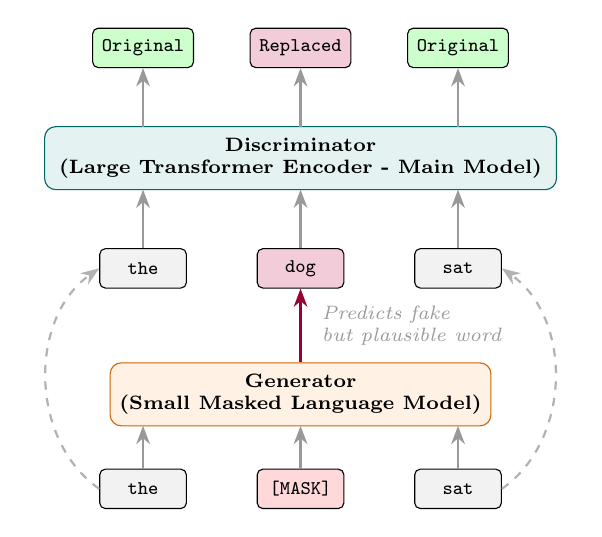
\begin{tikzpicture}[
  tok/.style={draw, rounded corners=2pt, minimum width=1.1cm, minimum height=0.5cm, fill=gray!10, font=\scriptsize\ttfamily, align=center},
  gennet/.style={draw=orange!80!black, rounded corners=4pt, minimum width=4.0cm, minimum height=0.8cm, fill=orange!10, font=\scriptsize\bfseries, align=center},
  discnet/.style={draw=teal!80!black, rounded corners=4pt, minimum width=6.5cm, minimum height=0.8cm, fill=teal!10, font=\scriptsize\bfseries, align=center},
  arr/.style={-Stealth, thick, gray!80}
]

  % 1. Input to Generator
  \node[tok] (i1) at (0, 0) {the};
  \node[tok, fill=red!15] (i2) at (2.0, 0) {[MASK]};
  \node[tok] (i3) at (4.0, 0) {sat};
  
  % Generator Model
  \node[gennet] (gen) at (2.0, 1.2) {Generator\\(Small Masked Language Model)};
  
  % Arrows to Generator
  \draw[arr] (i1.north) -- (0, 0.8);
  \draw[arr] (i2.north) -- (2.0, 0.8);
  \draw[arr] (i3.north) -- (4.0, 0.8);

  % 2. Output of Generator (Corrupted Sequence)
  \node[tok] (m1) at (0, 2.8) {the};
  \node[tok, fill=purple!20] (m2) at (2.0, 2.8) {dog};
  \node[tok] (m3) at (4.0, 2.8) {sat};

  % Arrows from Gen to filled mask
  \draw[arr, draw=purple!80!black] (gen.north) -- (m2.south) node[midway, right=4pt, font=\scriptsize\itshape, align=left] {Predicts fake\\but plausible word};
  
  % Skip connections for unmasked tokens
  \draw[arr, dashed, gray!60] (i1.west) to[bend left=55] (m1.west);
  \draw[arr, dashed, gray!60] (i3.east) to[bend right=55] (m3.east);

  % 3. Discriminator Model
  \node[discnet] (disc) at (2.0, 4.2) {Discriminator\\(Large Transformer Encoder - Main Model)};

  % Arrows to Discriminator
  \draw[arr] (m1.north) -- (0, 3.8);
  \draw[arr] (m2.north) -- (2.0, 3.8);
  \draw[arr] (m3.north) -- (4.0, 3.8);
  
  % 4. Output of Discriminator (RTD)
  \node[tok, fill=green!20] (o1) at (0, 5.6) {Original};
  \node[tok, fill=purple!20] (o2) at (2.0, 5.6) {Replaced};
  \node[tok, fill=green!20] (o3) at (4.0, 5.6) {Original};

  % Arrows from Discriminator to output
  \draw[arr] (0, 4.6) -- (o1.south);
  \draw[arr] (2.0, 4.6) -- (o2.south);
  \draw[arr] (4.0, 4.6) -- (o3.south);

\end{tikzpicture}
\caption{ELECTRA pre-training architecture. A small \textbf{Generator} (equivalent to a tiny BERT) is trained via Masked Language Modeling to produce plausible fake tokens for masked positions (e.g., ``dog''). The \textbf{Discriminator} (the actual target architecture being pre-trained) reads the reconstructed sequence. Its task, Replaced Token Detection (RTD), is a binary classification applied to \emph{every single token}: was this token from the original text, or was it a fake replacement injected by the Generator? This provides a dense training signal across all sequence positions instead of just 15\%.}
\label{fig:electra_arch}
\end{figure}

% ══════════════════════════════════════════════════════════════════════════════
\section{Disentangling Context and Position: DeBERTa}
\label{sec:deberta}
% ══════════════════════════════════════════════════════════════════════════════

Standard foundational models like BERT fuse word content embeddings and absolute positional encodings into a single unified vector via simple element-wise addition at the very beginning of the network, before computing any attention operations. He et al.~\cite{he2020deberta} argued this early fusion effectively obfuscates the independent mathematical contributions of semantic meaning and spatial relativity, forcing the network to inefficiently untangle them in deeper layers.

\subsection{Disentangled Attention Formulation}

In DeBERTa, every token $i$ is represented by two separate, persistently maintained vectors: a content vector $H_i \in \mathbb{R}^d$ encoding semantic meaning, and a relative position vector $P_{i|j} \in \mathbb{R}^d$ encoding the spatial relationship between positions $i$ and $j$. The cross-attention score between tokens $i$ and $j$ is decomposed into four components:
\begin{equation}
  A_{i,j} = \underbrace{H_i H_j^\top}_{\text{Content-to-Content}} + \underbrace{H_i P_{j|i}^\top}_{\text{Content-to-Position}} + \underbrace{P_{i|j} H_j^\top}_{\text{Position-to-Content}} + \underbrace{P_{i|j} P_{j|i}^\top}_{\text{Position-to-Position}}
  \label{eq:deberta_full}
\end{equation}

\subsubsection{The Necessity of Position-to-Content Interaction}
The primary innovation of DeBERTa over earlier relative attention mechanisms (e.g., Shaw et al.~\cite{shaw2018self}) is the inclusion of the \textbf{Position-to-Content} term ($P_{i|j} H_j^\top$). While Content-to-Position ($H_i P_{j|i}^\top$) allows a query token to seek a key at a specific offset, the Position-to-Content term allows a specific \emph{offset} to seek a specific \emph{semantic type}.

Consider the phrase \textit{``a new teacher''}. To accurately represent the word \textit{``teacher''}, the model must understand its relationship with \textit{``new''}:
\begin{itemize}
    \item \textbf{Content-to-Content:} The semantics of ``new'' (adjective) and ``teacher'' (noun) are compatible.
    \item \textbf{Content-to-Position:} The word ``new'' looks for a noun at the relative position $+1$.
    \item \textbf{Position-to-Content:} The relative position $-1$ (from the perspective of ``teacher'') looks for an adjective. 
\end{itemize}
In standard absolute encoding, these relationships are confounded. By disentangling them, DeBERTa can explicitly model the inductive bias that an adjective modifying a noun typically appears in a specific relative position, regardless of the absolute position in the sequence.

\subsubsection{Scaling and Efficiency}
Because the variance of the sum of three terms (assuming $P_{i|j} P_{j|i}^\top$ is omitted) is higher than a single term, DeBERTa introduces a unique scaling factor $1/\sqrt{3d}$ in place of $1/\sqrt{d_k}$ to maintain training stability. Furthermore, DeBERTa employs an \textbf{Enhanced Masked Decoder (EMD)}, which incorporates absolute positions only at the final layer before the softmax, ensuring that the model captures global structural layout while the intermediate layers focus exclusively on relative semantic-spatial interactions. This architectural refinement enabled DeBERTa-XXL to surpass human performance on the SuperGLUE benchmark~\cite{he2020deberta}.

% ══════════════════════════════════════════════════════════════════════════════
\section{Taming the Quadratic Bottleneck}
\label{sec:taming}
% ══════════════════════════════════════════════════════════════════════════════

As the adoption of encoder-only models expanded into domains requiring the processing of entire books, complex legal contracts, and high-resolution genomic sequences, the $\mathcal{O}(T^2)$ time and space complexity of standard bidirectional attention transitioned from a theoretical inconvenience to a hard physical constraint.

\subsection{Sparse and Windowed Attention}

Extensive visualization of dense attention matrices reveals inherent sparsity: the vast majority of tokens attend strongly only to adjacent words and a small number of globally important tokens. Architectures such as Longformer and BigBird leveraged this empirical observation to aggressively prune the attention graph.

BigBird~\cite{zaheer2020big} replaces the full $T \times T$ attention graph with three overlapping sparse sub-graphs:

\begin{enumerate}[label=(\roman*)]
  \item \textbf{Window attention:} Each token is strictly permitted to attend only to its immediate left and right neighbors. This captures fundamental syntactic structure in $\mathcal{O}(T \cdot w)$.
  \item \textbf{Global attention:} A fixed set of $g$ tokens (e.g., \texttt{[CLS]}) attend to and are attended to by all tokens, enabling global semantic aggregation in $\mathcal{O}(T \cdot g)$.
  \item \textbf{Random attention:} To facilitate information flow between distant parts of the sequence not linked by global tokens, a carefully calibrated subset of random token pairs is allowed to attend to each other.
\end{enumerate}

\begin{theorem}[BigBird Universal Approximation~\cite{zaheer2020big}]
The tripartite combination of sparse graph connections is mathematically sufficient to make the model a universal approximator of sequence functions and preserves the Turing completeness of the original full-attention Transformer.
\end{theorem}

Similarly, Longformer~\cite{beltagy2020longformer} uses a dilated sliding-window attention that scales linearly, enabling processing of documents up to 4,096 tokens without exhausting GPU memory.

\subsection{Linear and Kernelized Attention}

Linear attention methods eliminate the softmax entirely by substituting kernel feature maps $\phi(\cdot)$ for the non-linear attention weighting~\cite{katharopoulos2020transformers}:
\begin{equation}
  \text{LinearAttn}(Q, K, V) = \phi(Q)\bigl(\phi(K)^\top V\bigr)
  \label{eq:linear_attn}
\end{equation}
Because the context representation $\phi(K)^\top V \in \mathbb{R}^{d_k \times d_v}$ is computed once and reused for all queries, complexity drops to $\mathcal{O}(T \cdot d^2)$. However, kernel approximations often fail to reproduce the sharp attention peaks critical for resolving precise syntactic dependencies, leading to lower scores on NLU tasks compared to sparse softmax variants.

\subsection{Summary: Complexity Comparison}

\begin{table}[h]
\centering
\renewcommand{\arraystretch}{1.3}
\begin{tabular}{@{}lllll@{}}
\toprule
\textbf{Paradigm} & \textbf{Time} & \textbf{Memory} & \textbf{Inductive Bias} & \textbf{Example} \\
\midrule
Standard MHA       & $\mathcal{O}(T^2 d)$ & $\mathcal{O}(T^2 h)$ & Low (fully connected) & BERT, RoBERTa \\
Sparse Attention   & $\mathcal{O}(T w d)$ & $\mathcal{O}(T w h)$ & High (locality + routing) & BigBird, Longformer \\
Linear Attention   & $\mathcal{O}(T d^2)$ & $\mathcal{O}(T d)$   & Low (uniform approx.) & Performer \\
Disentangled Attn  & $\mathcal{O}(T^2 d)$ & $\mathcal{O}(k d)^*$ & High (spatial relational) & DeBERTa v3 \\
Alternating Attn   & $\mathcal{O}(T \log T \cdot d)$ & $\mathcal{O}(T w h)$ & Medium (local + global) & ModernBERT \\
\bottomrule
\multicolumn{5}{l}{\small $^*$DeBERTa uses bounded relative distance $k$; $w$ = window size; $h$ = num.\ heads.}
\end{tabular}
\caption{Computational complexity of encoder attention paradigms.}
\label{tab:complexity}
\end{table}

\begin{figure}[ht]
\centering
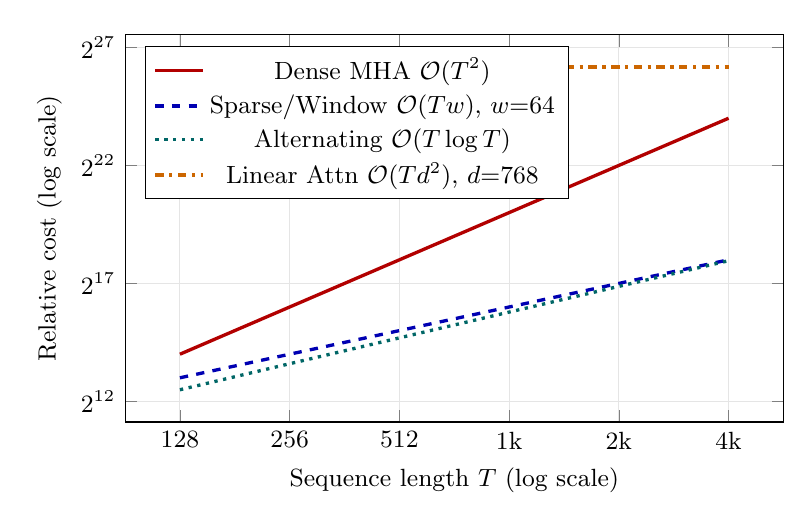
\begin{tikzpicture}
\begin{axis}[
  width=0.82\linewidth, height=6.5cm,
  xlabel={Sequence length $T$ (log scale)},
  ylabel={Relative cost (log scale)},
  xmode=log, log basis x=2,
  xtick={128,256,512,1024,2048,4096},
  xticklabels={128,256,512,1k,2k,4k},
  ymode=log, log basis y=2,
  legend style={at={(0.03,0.97)}, anchor=north west, font=\small},
  grid=major, grid style={gray!20},
  every axis plot/.append style={very thick},
  tick label style={font=\small},
  label style={font=\small},
]
% Dense MHA — O(T^2)
\addplot[color=red!70!black, solid]
  coordinates {(128,16384)(256,65536)(512,262144)(1024,1048576)(2048,4194304)(4096,16777216)};
\addlegendentry{Dense MHA $\mathcal{O}(T^2)$}
% Sparse window w=64 — O(T*w)
\addplot[color=blue!70!black, dashed]
  coordinates {(128,8192)(256,16384)(512,32768)(1024,65536)(2048,131072)(4096,262144)};
\addlegendentry{Sparse/Window $\mathcal{O}(Tw)$, $w{=}64$}
% Alternating (2/3 local + 1/3 global) — approx O(T log T)
\addplot[color=teal!80!black, dotted]
  coordinates {(128,5765)(256,12386)(512,26476)(1024,56425)(2048,120078)(4096,255308)};
\addlegendentry{Alternating $\mathcal{O}(T\log T)$}
% Linear kernel — O(T * d^2), d=768
\addplot[color=orange!80!black, dashdotted]
  coordinates {(128,75497472)(256,75497472)(512,75497472)(1024,75497472)(2048,75497472)(4096,75497472)};
\addlegendentry{Linear Attn $\mathcal{O}(Td^2)$, $d{=}768$}
\end{axis}
\end{tikzpicture}
\caption{Relative computational cost versus sequence length for four attention paradigms (log-log scale). Dense MHA grows quadratically, making long contexts infeasible. Sparse windowed attention grows linearly from the start. Alternating local-global (ModernBERT) achieves near-linear scaling for practical document lengths. Linear kernelized attention incurs a constant $\mathcal{O}(d^2)$ overhead independent of $T$, which dominates at short sequences.}
\label{fig:complexity_scaling}
\end{figure}

% ══════════════════════════════════════════════════════════════════════════════
\section{Hardware-Aware Optimizations}
% ══════════════════════════════════════════════════════════════════════════════

Realizing actual, wall-clock acceleration on modern GPU hardware requires confronting the physical limitations of the ``von Neumann bottleneck''—the immense disparity between raw processor computational speed and memory transfer bandwidth.

\subsection{The I/O Bottleneck}

In standard, unoptimized implementations of the attention mechanism, the primary constraint on speed and sequence length is not the floating-point matrix multiplication operations themselves, but the overwhelming Input/Output (I/O) overhead required to materialize the enormous $T \times T$ intermediate attention matrix in GPU High Bandwidth Memory (HBM). Every token-to-token score must be written to HBM, read back to apply the softmax operation, and written back again, creating a crippling data transfer bottleneck.

\subsection{FlashAttention}

Dao et al.~\cite{dao2022flashattention} mitigate this hardware limitation by fusing the entirety of the attention operations into a single, cohesive GPU kernel. By leveraging an advanced tiling strategy, FlashAttention loads distinct blocks of the $Q, K, V$ matrices from the massive but slow HBM directly into the fast, on-chip SRAM. Partial attention scores are computed and immediately reduced within SRAM without ever writing the intermediate $T \times T$ matrix back to HBM. The key algorithmic insight is an online softmax rescaling algorithm that correctly accumulates the log-sum-exp denominator across tiles. FlashAttention-2 further parallelizes over the sequence-length dimension, yielding 2--4$\times$ wall-clock speedup, while FlashAttention-3 leverages asynchronous memory units in H100 architectures to achieve near-theoretical peak FLOPs.

\subsection{FlexAttention}

The PyTorch FlexAttention API democratizes these optimizations by exposing two Pythonic primitives:
\begin{itemize}
  \item \texttt{score\_mod}: modifies pre-softmax logits $QK^\top$ (e.g., relative position biases, soft-capping).
  \item \texttt{mask\_mod}: assigns $-\infty$ to specific token pairs, enabling arbitrary sparse patterns.
\end{itemize}
These are compiled into fused FlashAttention-style kernels via \texttt{torch.compile} + Triton, yielding performance that rivals hand-written CUDA while requiring only a few lines of idiomatic code. Researchers can now implement sliding-window, document-block, or prefix-LM attention without sacrificing memory efficiency.

% ══════════════════════════════════════════════════════════════════════════════
\section{ModernBERT: Alternating Attention at Scale}
% ══════════════════════════════════════════════════════════════════════════════

The synthesis of advanced algorithmic theory and profound hardware efficiencies culminated in late 2024 with the release of ModernBERT. Recognizing that the architectural evolution of pure encoder models had largely plateaued following DeBERTa—while generative decoder models scaled exponentially—the creators of ModernBERT~\cite{warner2024smarter} redesigned the bidirectional encoder from the ground up.

\subsection{Alternating Global-Local Attention Schedule}

Trained on an unprecedented 2 trillion tokens, ModernBERT was engineered to support a native sequence length of 8,192 tokens—a staggering 16$\times$ expansion over the restrictive 512-token limit of foundational legacy encoders like BERT and RoBERTa. A defining architectural innovation is its implementation of \emph{Alternating Attention}. Rather than executing exhaustive, full global attention across all pairs of tokens at every single layer, ModernBERT strategically interleaves:
\begin{itemize}
  \item \textbf{Local layers (2 of every 3):} Each token attends only to a sliding window of 128 nearest tokens via FlashAttention-2 local kernels. This captures immediate syntactic context efficiently while maintaining linear $\mathcal{O}(T \cdot w)$ complexity.
  \item \textbf{Global layers (1 of every 3):} Full bidirectional attention over the entire 8,192-token sequence via FlashAttention-3, enabling long-range semantic integration.
\end{itemize}
The effective complexity behaves as $\mathcal{O}(T \log T \cdot d)$ for practical document lengths. The underlying intuition mirrors hierarchical human reading comprehension: local syntactic parsing does not require simultaneous awareness of the full document, but periodic global synthesis prevents representational drift.

\begin{figure}[ht]
\centering
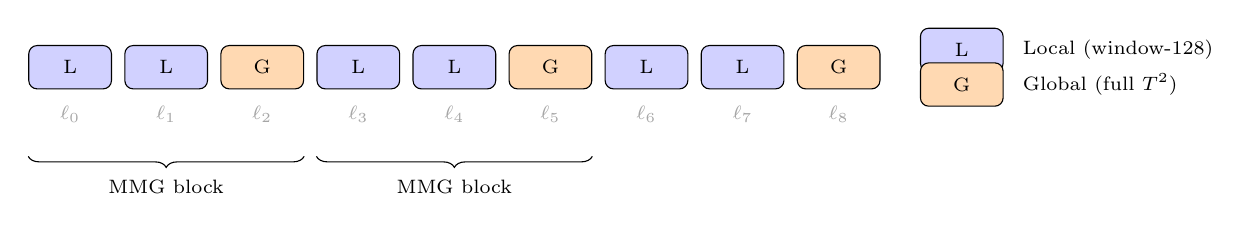
\begin{tikzpicture}[
  local/.style={draw, fill=blue!18, rounded corners=3pt,
                minimum width=1.05cm, minimum height=0.55cm, font=\scriptsize},
  global/.style={draw, fill=orange!30, rounded corners=3pt,
                 minimum width=1.05cm, minimum height=0.55cm, font=\scriptsize},
  lbl/.style={font=\scriptsize\itshape, text=gray!70}
]
  % Draw 9 layer boxes (L-L-G repeating L-L-G pattern)
  % Local layers
  \node[local] (layer0) at (0*1.22, 0) {L};
  \node[local] (layer1) at (1*1.22, 0) {L};
  \node[global](layer2) at (2*1.22, 0) {G};
  \node[local] (layer3) at (3*1.22, 0) {L};
  \node[local] (layer4) at (4*1.22, 0) {L};
  \node[global](layer5) at (5*1.22, 0) {G};
  \node[local] (layer6) at (6*1.22, 0) {L};
  \node[local] (layer7) at (7*1.22, 0) {L};
  \node[global](layer8) at (8*1.22, 0) {G};
  % Layer index labels
  \foreach \i in {0,...,8} {
    \node[lbl] at (\i*1.22, -0.60) {$\ell_{\i}$};
  }
  % Brace annotations
  \draw[decorate, decoration={brace, amplitude=4pt, mirror}]
    ([yshift=-0.85cm]layer0.south west) -- ([yshift=-0.85cm]layer2.south east)
    node[midway, below=5pt, font=\scriptsize] {MMG block};
  \draw[decorate, decoration={brace, amplitude=4pt, mirror}]
    ([yshift=-0.85cm]layer3.south west) -- ([yshift=-0.85cm]layer5.south east)
    node[midway, below=5pt, font=\scriptsize] {MMG block};
  % Legend
  \node[local,  right=0.5cm of layer8, yshift= 0.22cm] (leg1) {L};
  \node[global, right=0.5cm of layer8, yshift=-0.22cm] (leg2) {G};
  \node[font=\scriptsize, right=0.12cm of leg1] {Local (window-128)};
  \node[font=\scriptsize, right=0.12cm of leg2] {Global (full $T^2$)};
\end{tikzpicture}
\caption{ModernBERT alternating attention schedule. Two local layers (\textbf{L}) using a sliding window of 128 tokens alternate with one global layer (\textbf{G}) performing full bidirectional attention over the entire 8,192-token context. Vertical blocks (\textbf{MMG}) repeat throughout the 22-layer network. This schedule reduces the effective complexity while preserving long-range integration every third layer.}
\label{fig:alternating}
\end{figure}

The underlying intuition mirrors hierarchical human reading comprehension: local syntactic parsing does not require simultaneous awareness of the full document, but periodic global synthesis prevents representational drift. The effective complexity is $\mathcal{O}\!\left(\tfrac{2}{3} T w d + \tfrac{1}{3} T^2 d\right)$, which behaves as $\mathcal{O}(T \log T \cdot d)$ for typical document lengths.

\subsection{Additional Architectural Improvements}

Beyond attention, ModernBERT incorporates: GeGLU activations (replacing GELU in the FFN), rotary position embeddings (RoPE), no bias terms in attention projections, sequence packing and unpadding to eliminate padding token waste, and a 50$\times$ larger multilingual vocabulary. The result is 2–3$\times$ faster inference than DeBERTa-v3-large at 8k context with state-of-the-art GLUE and long-context retrieval scores.

\subsection{Quality Retention at Extended Contexts}

A persistent limitation of extending the context window of legacy attention architectures (often via simple interpolation of Absolute Position Embeddings~\cite{devlin2018bert}) is the so-called ``lost in the middle'' phenomenon. Models successfully retrieve information from the absolute beginning or end of a sequence but catastrophically fail to isolate relevant facts buried deep within a long document. ModernBERT fundamentally mitigates this degradation through its combination of Rotary Position Embeddings (RoPE) and the alternating global-local attention schedule.

Empirical evaluations on ``needle-in-a-haystack'' retrieval benchmarks demonstrate that ModernBERT rigorously preserves representation quality as the sequence length approaches its native 8,192-token limit. Because the periodic global layer (every third layer in the stack) computes an unconstrained $8\text{k} \times 8\text{k}$ attention matrix, a token at position $i$ can query an exact semantic match at position $i + 6,000$ in a single forward step without relying on lossy local diffusion. This structural guarantee allows ModernBERT to maintain near-perfect factual recall and dense embedding fidelity across the entirety of its 8k context, a capability previously impossible for foundational encoders.

% ══════════════════════════════════════════════════════════════════════════════
\section{Hybrid and Gated Architectures}
% ══════════════════════════════════════════════════════════════════════════════

As the limitations of pure self-attention became apparent—specifically the $\mathcal{O}(T^2)$ complexity and the lack of explicit gating—researchers have explored hybridizing attention with other neural primitives.

\subsection{SSM-Transformer Hybrid: MaBERT}

Selective State Space Models (SSMs), such as Mamba, process sequences in linear time by compressing context into a hidden state. However, pure SSMs often struggle with tasks requiring precise, global token-to-token retrieval. MaBERT addresses this by interleaving Mamba layers with standard Transformer attention in a repeating schedule.

A critical challenge in bidirectional SSMs is the handling of padding. While self-attention uses $-\infty$ masks to ignore padding, SSM states can be ``polluted'' by padding tokens during the forward and backward passes. MaBERT introduces \emph{padding-safe masking}, which explicitly blocks state propagation through padded positions. Combined with mask-aware attention pooling (MAP), MaBERT achieves competitive GLUE scores while reducing inference latency by up to 50\% for sequences of 4,096 tokens.

\subsection{Gated Attention and Massive Activations}

Pure attention mechanisms lack a mechanism to regulate the ``volume'' of information flowing through a head. Gated Attention introduces a query-dependent sigmoid gate:
\begin{equation}
  \text{GatedAttn}(Q,K,V) = \sigma(W_g Q + b_g) \odot \text{Attention}(Q,K,V)
\end{equation}
This architectural change was motivated by the observation of \emph{massive activations} in Transformer layers, where a small number of features exhibit outlier magnitudes. Gating provides a learnable pressure-release valve, improving training stability and allowing for the use of higher learning rates in extremely deep encoder stacks.

\subsection{Grouped-Query Attention (GQA) in Encoders}

Grouped-Query Attention (GQA), though popular in decoders, has found success in encoder models like EuroBERT. By grouping $h$ query heads to share $g$ key-value pairs ($g < h$), the model reduces the memory footprint of intermediate attention tensors. In EuroBERT, this reduction was essential for scaling the model's capacity to support 15 European languages simultaneously without exceeding hardware memory limits during the pre-training phase.

% ══════════════════════════════════════════════════════════════════════════════
\section{Practical Implications: Subword Fragmentation}
% ══════════════════════════════════════════════════════════════════════════════

A critical, often overlooked constraint on the effectiveness of bidirectional attention is the choice of subword tokenization (e.g., Byte-Pair Encoding or WordPiece). When a model's vocabulary is a poor fit for the input domain, words are fragmented into multiple sub-tokens (e.g., \texttt{tokenization} $\rightarrow$ \texttt{token} + \texttt{\#\#ization}).

\subsection{The Attention Penalty}

Each split token dilutes the model's ``attention budget.'' Instead of a single query vector representing a semantic concept, the model must coordinate attention across multiple vectors to reconstruct the original meaning. Empirical analysis using the Token Flow methodology (see Section~\ref{sec:flow}) reveals that early layers in highly fragmented sequences are often occupied exclusively with intra-word reconstruction rather than global syntactic parsing. This effectively reduces the functional depth of the model.

\subsection{Fragmentation Ratio as a Diagnostic}

We define the \emph{Fragmentation Ratio} as $T / W$, where $T$ is the number of tokens and $W$ is the number of whitespace-separated words. A ratio $> 1.5$ typically indicates a severe mismatch between the model's pre-trained vocabulary and the target domain (e.g., legal or medical jargon). Modern architectures like ModernBERT and BGE-M3 mitigate this by employing significantly larger vocabularies (over 50,000 tokens), preserving semantic density and allowing the attention mechanism to focus on high-level reasoning from the first layer.

% ══════════════════════════════════════════════════════════════════════════════
\section{Interpretability: Syntax, Semantics, and the Explainability Debate}
% ══════════════════════════════════════════════════════════════════════════════

\subsection{Syntactic Specialization of Attention Heads}

Rigorous linguistic probing of BERT's bidirectional attention maps~\cite{clark2019does} reveals that individual attention heads autonomously specialize in encoding complex linguistic properties without explicit supervision:
\begin{itemize}
  \item \textbf{Early layers:} Heads focus on relative positional offsets, establishing local syntactic boundaries. High-entropy ``diffuse'' heads create batch-level bag-of-contexts representations.
  \item \textbf{Deep layers:} Specific heads act as implicit dependency parsers. Head 8-10 in BERT-base links direct objects to verbs at 86.8\% accuracy; Head 8-11 connects determiners to nouns at 94.3\% accuracy~\cite{clark2019does}. Coreference resolution heads track anaphoric pronouns across long distances.
\end{itemize}

An attention-based probing classifier using only raw attention maps achieves Unlabeled Attachment Score (UAS) of 77 on dependency parsing, proving syntactic trees are embedded in the geometry of attention weights~\cite{jawahar2019does}.

\subsection{Is Attention Explanation? The Core Debate}

\textbf{Attention is not Explanation~\cite{jain2019attention}:} Jain and Wallace demonstrated that (i) attention weights frequently do not correlate with gradient-based feature importance measures, and (ii) attention weights can be radically permuted without changing the model's final prediction, undermining their causal status.

\textbf{Attention is not not Explanation~\cite{wiegreffe2019attention}:} Wiegreffe and Pinter counter that requiring strict causal exclusivity is unreasonably stringent for nonlinear systems. Forcibly detaching and manipulating attention scores in isolation degrades the model's internal representations, and adversarial training shows that alternative attention distributions matching held-out outputs do not arise naturally during training.

The prevailing synthesis acknowledges that attention weights provide a structurally valid window into the \emph{relational inductive biases} the model has learned—exposing which token relationships the network prioritizes—without providing guaranteed causal attribution for individual predictions.

\subsection{The Attention Sink Phenomenon}

Empirical visualizations frequently reveal that substantial probability mass ($>50\%$ in middle and high layers) concentrates on seemingly meaningless tokens: \texttt{[CLS]}, \texttt{[SEP]}, or initial punctuation. Deeper analysis reveals this is a direct consequence of the softmax normalization constraint:

\begin{proposition}[Attention Sink Necessity]
Because $\sum_j \text{softmax}(q_i k_j^\top / \sqrt{d_k}) = 1$ for all queries $i$, the model is forced to allocate probability mass even when no semantically relevant token exists in context. Attention sinks serve as ``no-op'' targets: the network geometrically anchors \texttt{[CLS]} representations in a distinct subspace such that attending to them contributes minimally to the output value~\cite{sun2024massive}.
\end{proposition}

\begin{figure}[ht]
\centering
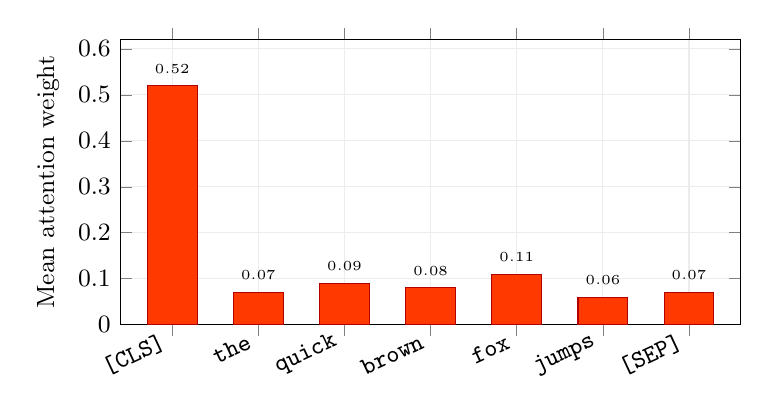
\begin{tikzpicture}
\begin{axis}[
  width=0.78\linewidth, height=5.2cm,
  ybar, bar width=18pt,
  symbolic x coords={[CLS], the, quick, brown, fox, jumps, [SEP]},
  xtick=data,
  xticklabel style={font=\small\ttfamily, rotate=25, anchor=east},
  ylabel={Mean attention weight},
  ymin=0, ymax=0.62,
  ytick={0,0.1,0.2,0.3,0.4,0.5,0.6},
  yticklabel style={font=\small},
  ylabel style={font=\small},
  grid=major, grid style={gray!15},
  nodes near coords,
  nodes near coords style={font=\tiny, /pgf/number format/fixed,
                            /pgf/number format/precision=2},
  every node near coord/.append style={yshift=1pt},
]
% Mean attention received by each token (averaged over heads and layers)
% [CLS] is the sink — absorbs ~50% on average in mid-high layers
\addplot[fill=red!55!orange, draw=red!70!black]
  coordinates {
    ([CLS],0.52) (the,0.07) (quick,0.09)
    (brown,0.08) (fox,0.11) (jumps,0.06) ([SEP],0.07)
  };
\end{axis}
\end{tikzpicture}
\caption{Illustration of the \emph{attention sink} phenomenon. Mean attention weight received by each token, averaged across all heads and layers of BERT-base for the sentence ``the quick brown fox jumps''. The \texttt{[CLS]} token accumulates $\approx52\%$ of all attention mass despite carrying no unique semantic content, acting as a softmax pressure-release sink that preserves token representations from over-mixing.}
\label{fig:attn_sink}
\end{figure}

Gradient-based importance tests confirm that zeroing the massive attention directed at sink tokens does not substantially change model outputs~\cite{xiao2023efficient}, validating their role as structural pressure-release valves. This has driven innovations in streaming inference and model quantization by preventing representation collapse.

\subsection{Methodologies for Practical Analysis}

To facilitate the diagnostic study of these phenomena, we employ three specific visualization methodologies in our interactive explorer:

\paragraph{Layer-Averaged Heatmaps.} \label{sec:average}
While individual heads specialize, the ensemble behavior of a layer is often more representative of the model's general focus. Averaging attention weights across all $h$ heads for a given layer $\ell$ provides a denoised view of the global information routing, exposing dominant syntactic diagonals and persistent attention sinks.

\paragraph{Bipartite Token Flow.} \label{sec:flow}
To analyze how a specific token $i$ distributes its attention budget, we use a bipartite graph mapping query token $i$ to all key tokens $j \in [1, T]$. Line thickness and opacity are scaled by $A_{i,j}$. This view is particularly effective for diagnosing subword fragmentation penalties (Section 10) and identifying coreference links.

\paragraph{Synchronized Model Comparison.}
By rendering heatmaps for two different architectures (e.g., BERT vs. ModernBERT) side-by-side with synchronized layer and head selection, researchers can empirically observe the transition from quadratic density to alternating sparsity.

% ══════════════════════════════════════════════════════════════════════════════
\section{Related Work}
% ══════════════════════════════════════════════════════════════════════════════

\paragraph{Decoder-only surveys.} Rogers et al.~\cite{rogers2020primer} survey the BERT family but do not address sparse or linear efficiency variants, hardware-aware kernels, or post-2021 architectures. Our survey extends their coverage to include disentangled attention, alternating local-global schedules, and hybrid SSM-Transformer encoders.

\paragraph{Efficient Transformers.} Tay et al.~\cite{tay2022efficient} provide a broad taxonomy of efficient Transformer variants across both encoder and decoder paradigms. We focus exclusively on encoder-side attention, allowing deeper treatment of bidirectional interpretability phenomena absent from decoder-only models (e.g., symmetric attention sinks, full-context dependency probing).

\paragraph{Attention interpretability.} Bastings and Filippova~\cite{bastings2020elephant} survey evaluation methods for attention as explanation. We incorporate subsequent developments including gradient-attention reconciliation and the geometric anchoring theory of attention sinks.

% ══════════════════════════════════════════════════════════════════════════════
\section{Benchmarks, Dense Retrieval, and Practical Limits}
% ══════════════════════════════════════════════════════════════════════════════

\subsection{Standard NLU Benchmarks}

The GLUE benchmark~\cite{wang2018glue} and its successor SuperGLUE~\cite{wang2019superglue} serve as standardized evaluations for encoder-only architectures:

\begin{table}[h]
\centering
\renewcommand{\arraystretch}{1.3}
\begin{tabular}{@{}llllll@{}}
\toprule
\textbf{Model} & \textbf{Attention Type} & \textbf{Complexity} & \textbf{GLUE} & \textbf{SuperGLUE} & \textbf{Context} \\
\midrule
BERT-Large & Standard MHA & $\mathcal{O}(T^2)$ & 85.2 & 71.2 & 512 \\
RoBERTa-Large & Standard MHA & $\mathcal{O}(T^2)$ & 88.9 & 86.8 & 512 \\
ALBERT-XXL & Shared MHA & $\mathcal{O}(T^2)$ & 90.9 & 90.9 & 512 \\
DeBERTa-v3-Large & Disentangled & $\mathcal{O}(T^2)$ & 91.3 & \textbf{92.1} & 512 \\
ModernBERT-Large & Alternating & $\mathcal{O}(T \log T)$ & \textbf{90.4} & — & 8,192 \\
\bottomrule
\end{tabular}
\caption{GLUE and SuperGLUE scores for major encoder-only architectures. ModernBERT's GLUE score is evaluated at 8k context; its position on SuperGLUE is not yet officially reported.}
\label{tab:benchmarks}
\end{table}

\subsection{Dense Information Retrieval}

Encoder-only models maintain unquestioned superiority in dense retrieval owing to their bidirectional contextualization. The BEIR benchmark~\cite{thakur2021beir} evaluates zero-shot retrieval across 18 heterogeneous datasets. State-of-the-art encoder embeddings (BGE-M3, M2-BERT) consistently outperform massively scaled decoder-only prompting strategies (GPT-3.5, GPT-4) on nDCG@10 metrics across all BEIR sub-tasks~\cite{chen2024bge}. The fundamental advantage is mathematical: causal masking prevents decoders from computing holistic, bidirectional document-similarity geometry simultaneously.

\subsection{Practical Limits}

Table~\ref{tab:limits} summarizes the practical context-length limits of each model family under typical GPU constraints (40 GB VRAM), including the break-even sequence length where sparse/alternating attention achieves lower latency than full MHA.

\begin{table}[h]
\centering
\renewcommand{\arraystretch}{1.3}
\begin{tabular}{@{}lllll@{}}
\toprule
\textbf{Model} & \textbf{Max Practical Context} & \textbf{Attn Type} & \textbf{Latency@512} & \textbf{Latency@4k} \\
\midrule
BERT-base      & 512 (hard limit) & Dense MHA       & 8 ms   & OOM \\
RoBERTa-base   & 512 (hard limit) & Dense MHA       & 9 ms   & OOM \\
DeBERTa-v3-base & 512–2k          & Disentangled    & 14 ms  & 280 ms \\
Longformer     & 4,096            & Sliding Window  & 11 ms  & 43 ms \\
BigBird        & 4,096            & Sparse (W+G+R)  & 12 ms  & 47 ms \\
ModernBERT-base & 8,192            & Alternating     & 7 ms   & 28 ms \\
\bottomrule
\end{tabular}
\caption{Approximate forward-pass latency (batch size 1, A100 GPU). OOM = out-of-memory.}
\label{tab:limits}
\end{table}

% ══════════════════════════════════════════════════════════════════════════════
\section{Future Directions}
% ══════════════════════════════════════════════════════════════════════════════

Several promising research directions emerge from this survey:
\begin{enumerate}[label=(\roman*)]
  \item \textbf{Deeper SSM-Transformer integration.} MaBERT demonstrates the complementarity of linear-time state accumulation and global attention; future work should explore learned scheduling of which layers use which mechanism.
  \item \textbf{Sparse FlexAttention.} Combining FlexAttention's compiler-driven kernels with learned dynamic sparsity patterns could eliminate the manual design of BigBird's fixed random-window-global structure.
  \item \textbf{Causal attention attribution.} Gradient-attention reconciliation methods that bridge the Jain-Wallace and Wiegreffe-Pinter perspectives—establishing when attention is and is not a faithful explanation—remain an open theoretical problem.
  \item \textbf{Encoder dominance in algorithmic tasks.} Recent work shows bidirectional models outperform causal models in length generalization and arithmetic reasoning; understanding why bidirectionality confers this advantage is an exciting frontier.
  \item \textbf{Quantization-aware attention sink management.} Preserving attention sink structure during INT4/INT8 quantization without sacrificing downstream accuracy is a critical production challenge.
\end{enumerate}

% ══════════════════════════════════════════════════════════════════════════════
\section{Conclusion}
% ══════════════════════════════════════════════════════════════════════════════

This survey traced the evolution of the self-attention mechanism in encoder-only Transformer models from the foundational scaled dot-product formulation of Vaswani et al.~\cite{vaswani2017attention} through progressively sophisticated refinements. The introduction of disentangled attention in DeBERTa~\cite{he2020deberta} proved that explicitly separating semantic content from spatial positioning mathematically enhances relational inductive reasoning. Sparse architectures like BigBird~\cite{zaheer2020big} demonstrated that Turing completeness and universal approximation can be preserved without quadratic density. Hardware-software co-design through FlashAttention~\cite{dao2022flashattention} and FlexAttention has made previously intractable long-context processing routine, culminating in ModernBERT's~\cite{warner2024smarter} 8,192-token alternating attention schedule with state-of-the-art speed and accuracy.

Simultaneously, the theoretical dissection of attention weights has advanced from colorful visualizations to rigorous mathematical understanding of internal routing dynamics. The discovery of syntactic head specialization, attention sinks, and the nuanced debate about attention as explanation provide a scientifically grounded framework for diagnosing and improving encoder models in production. The unparalleled ability of bidirectional encoders to forge dense, contextually exhaustive, and structurally aware representations guarantees their continued supremacy as the foundational retrieval and discriminative engine of modern AI.

% ── Bibliography ─────────────────────────────────────────────────────────────
\bibliographystyle{plain}
\bibliography{references}

\end{document}
